\documentclass[11pt]{article}

\usepackage[margin=1in]{geometry}
\usepackage{booktabs}
\usepackage{graphicx}
\usepackage{subcaption}
\usepackage{amsmath}
\usepackage[hidelinks]{hyperref}
\usepackage{xcolor}
\usepackage{enumitem}
\usepackage{microtype}

\graphicspath{{figures/}}

\title{MazeEval-Style Evidence for Strategy Degradation in Shared-Experience MAS}
\author{Draft experimental section}
\date{\today}

\begin{document}
\maketitle

\begin{abstract}
This draft section reports the current MazeEval-style pilot for studying strategy degradation in multi-agent systems (MAS) with shared experience. The central hypothesis is not that erroneous memories contaminate later reasoning, but that locally valid strategies can be amplified by consensus-driven writing, retrieval, and reuse until the system exhibits global inefficiency, route homogenization, and no-error loops. The current pilot shows that shared experience is not inherently harmful: reviewer-written shared memory can improve short-horizon performance. However, direct or oracle-style shared memories with high retrieval concentration produce higher path cost, higher loop rate, and later-stage collapse under a longer feedback horizon.
\end{abstract}

\section{Experimental Goal}

We study whether shared-experience MAS can turn locally reasonable strategies into globally inefficient behavior through positive feedback. This differs from an error-contamination account: the problematic memories are often semantically correct, such as ``avoid revisits'' or ``submit immediately once the goal is reached.'' The failure mode is that such strategies can be repeatedly retrieved, compressed, and reused without preserving enough information about their provenance or context. In the maze setting, this appears as legal movement, no wall crossing, and often successful completion, but with excessive path length, repeated visits, and loop-like motion.

\section{Benchmark Design}

We use a controlled MazeEval-style benchmark rather than a static full-map planning benchmark. Each agent receives local observations, including current position, goal position, open directions, distance-to-wall feedback, recent path history, visited/tried directions, and retrieved experience. Agents do not receive the hidden maze graph or the shortest path. The environment enforces movement semantics: attempted wall-crossing is blocked and logged as an invalid move, and success requires submitting at the goal cell.

The pilot uses $15 \times 15$ trap-family mazes with minimum shortest path length at least 30. Heldout mazes are fixed within a seed so that conditions can be compared on the same tasks, while training mazes feed the experience-writing loop. Each condition runs four homogeneous solver agents with the same model and prompt family. The key experimental variable is the memory mechanism.

\section{Experience Extraction and Collection}

The experience module is deliberately not a maze-specific rule engine. We follow the common design pattern used by ExpeL- and Reflexion-style agents: after an episode, the system converts trajectories, outcomes, and quality signals into reusable natural-language experiences, then retrieves those experiences in later episodes. For the multi-agent conditions, we use a MAEL-like organization in which multiple agents can contribute trajectories to either private memory pools or a shared global memory pool. The maze code only provides a task adapter: it formats the trajectory, observable feedback, and quality fields for the generic experience writer.

Each written experience is a short \emph{do/avoid} strategy lesson. The writer is instructed to contrast successful and inefficient trajectories, preserve strategy-level lessons, and avoid task answers. In particular, it may write abstract guidance such as ``after backtracking to the same junction, prefer an untried open direction'', but it must not write maze identifiers, coordinates, complete paths, or fixed action scripts. A sanitizer rejects over-specific memories, including coordinate-like text and long direction sequences, so the memory cannot become a route cache.

In the single-agent ExpeL calibration, one solver produces trajectories over training mazes and the reviewer writes experiences from that solver's own logs. This arm asks whether the experience-learning mechanism is useful in the maze family before introducing multi-agent sharing. In the MAS conditions, each homogeneous solver agent acts in an independent copy of the same maze. The reviewer sees only the agents' execution logs and quality summaries such as success, steps, invalid moves, revisits, stagnation, and loop flags; it does not receive the hidden maze graph or a solution path. Private-memory conditions write each agent's lessons to its own pool, while shared-memory conditions merge lessons into a global pool retrieved by all agents.

We also include direct and oracle write modes as ablations. They are not the main claim about mainstream MAS, but they isolate what happens when a small number of correct abstract strategy memories dominate retrieval. The audit file records every memory's source episode, writer mode, support count, retrieval count, and downstream usage, which lets us distinguish memory content from memory provenance.

\section{Conditions}

\begin{description}[leftmargin=2.2cm, style=nextline]
    \item[Frozen] Experience is written but never retrieved. This isolates storage from active memory injection.
    \item[Private fixed] Each agent writes to and retrieves from its own private memory pool. This tests whether experience helps without global sharing.
    \item[Shared reviewer] A reviewer summarizes agent trajectories into shared natural-language experiences. This is the closest condition to mainstream MAS experience-sharing.
    \item[Shared direct] A small set of direct strategy memories is written from trajectory outcomes and shared globally.
    \item[Shared oracle] A small set of oracle/success-based strategy memories is written globally. The content is correct at the abstract level, but can still become over-concentrated during retrieval.
\end{description}

\section{Metrics}

We report success rate, cost ratio, loop rate, route diversity, memory size, and retrieval concentration. Cost ratio is
\[
    \mathrm{cost\_ratio} = \frac{\mathrm{actual\_steps}}{\mathrm{shortest\_path\_length}},
\]
where the shortest path is used only by the evaluator and is not shown to agents. Loop rate flags short repeated position cycles or repeated-cell behavior without progress. Route diversity measures variation in the visited routes across agents. Retrieval concentration measures whether agents increasingly retrieve the same few memories.

\section{Main Matrix: Short-Horizon Memory Feedback}

Table~\ref{tab:full-matrix} reports the final round of the $T=3$, three-seed full matrix. The frozen control is stable because it never retrieves written memories. Private memory preserves diversity and is roughly comparable to frozen. Shared reviewer obtains the best short-horizon outcome: success reaches 1.000, cost is lowest, and loop rate is lowest. However, its route diversity is also lowest, showing that it compresses behavior into more homogeneous routes. In contrast, shared direct and shared oracle have high retrieval concentration and substantially higher cost.

\begin{table}[h]
\centering
\caption{Final mean metrics for the $T=3$ full matrix, averaged over three seeds.}
\label{tab:full-matrix}
\begin{tabular}{lrrrrrr}
\toprule
Condition & Success & Cost & Loop & Diversity & Memory & Retrieval conc. \\
\midrule
Frozen          & 0.944 & 2.334 & 0.056 & 0.177 & 8.0  & 0.000 \\
Private fixed   & 0.972 & 2.348 & 0.056 & 0.232 & 31.3 & 0.051 \\
Shared reviewer & 1.000 & 2.179 & 0.028 & 0.139 & 8.0  & 0.206 \\
Shared direct   & 0.917 & 3.092 & 0.139 & 0.277 & 1.7  & 0.804 \\
Shared oracle   & 0.944 & 3.042 & 0.083 & 0.236 & 2.0  & 0.783 \\
\bottomrule
\end{tabular}
\end{table}

\begin{figure}[h]
\centering
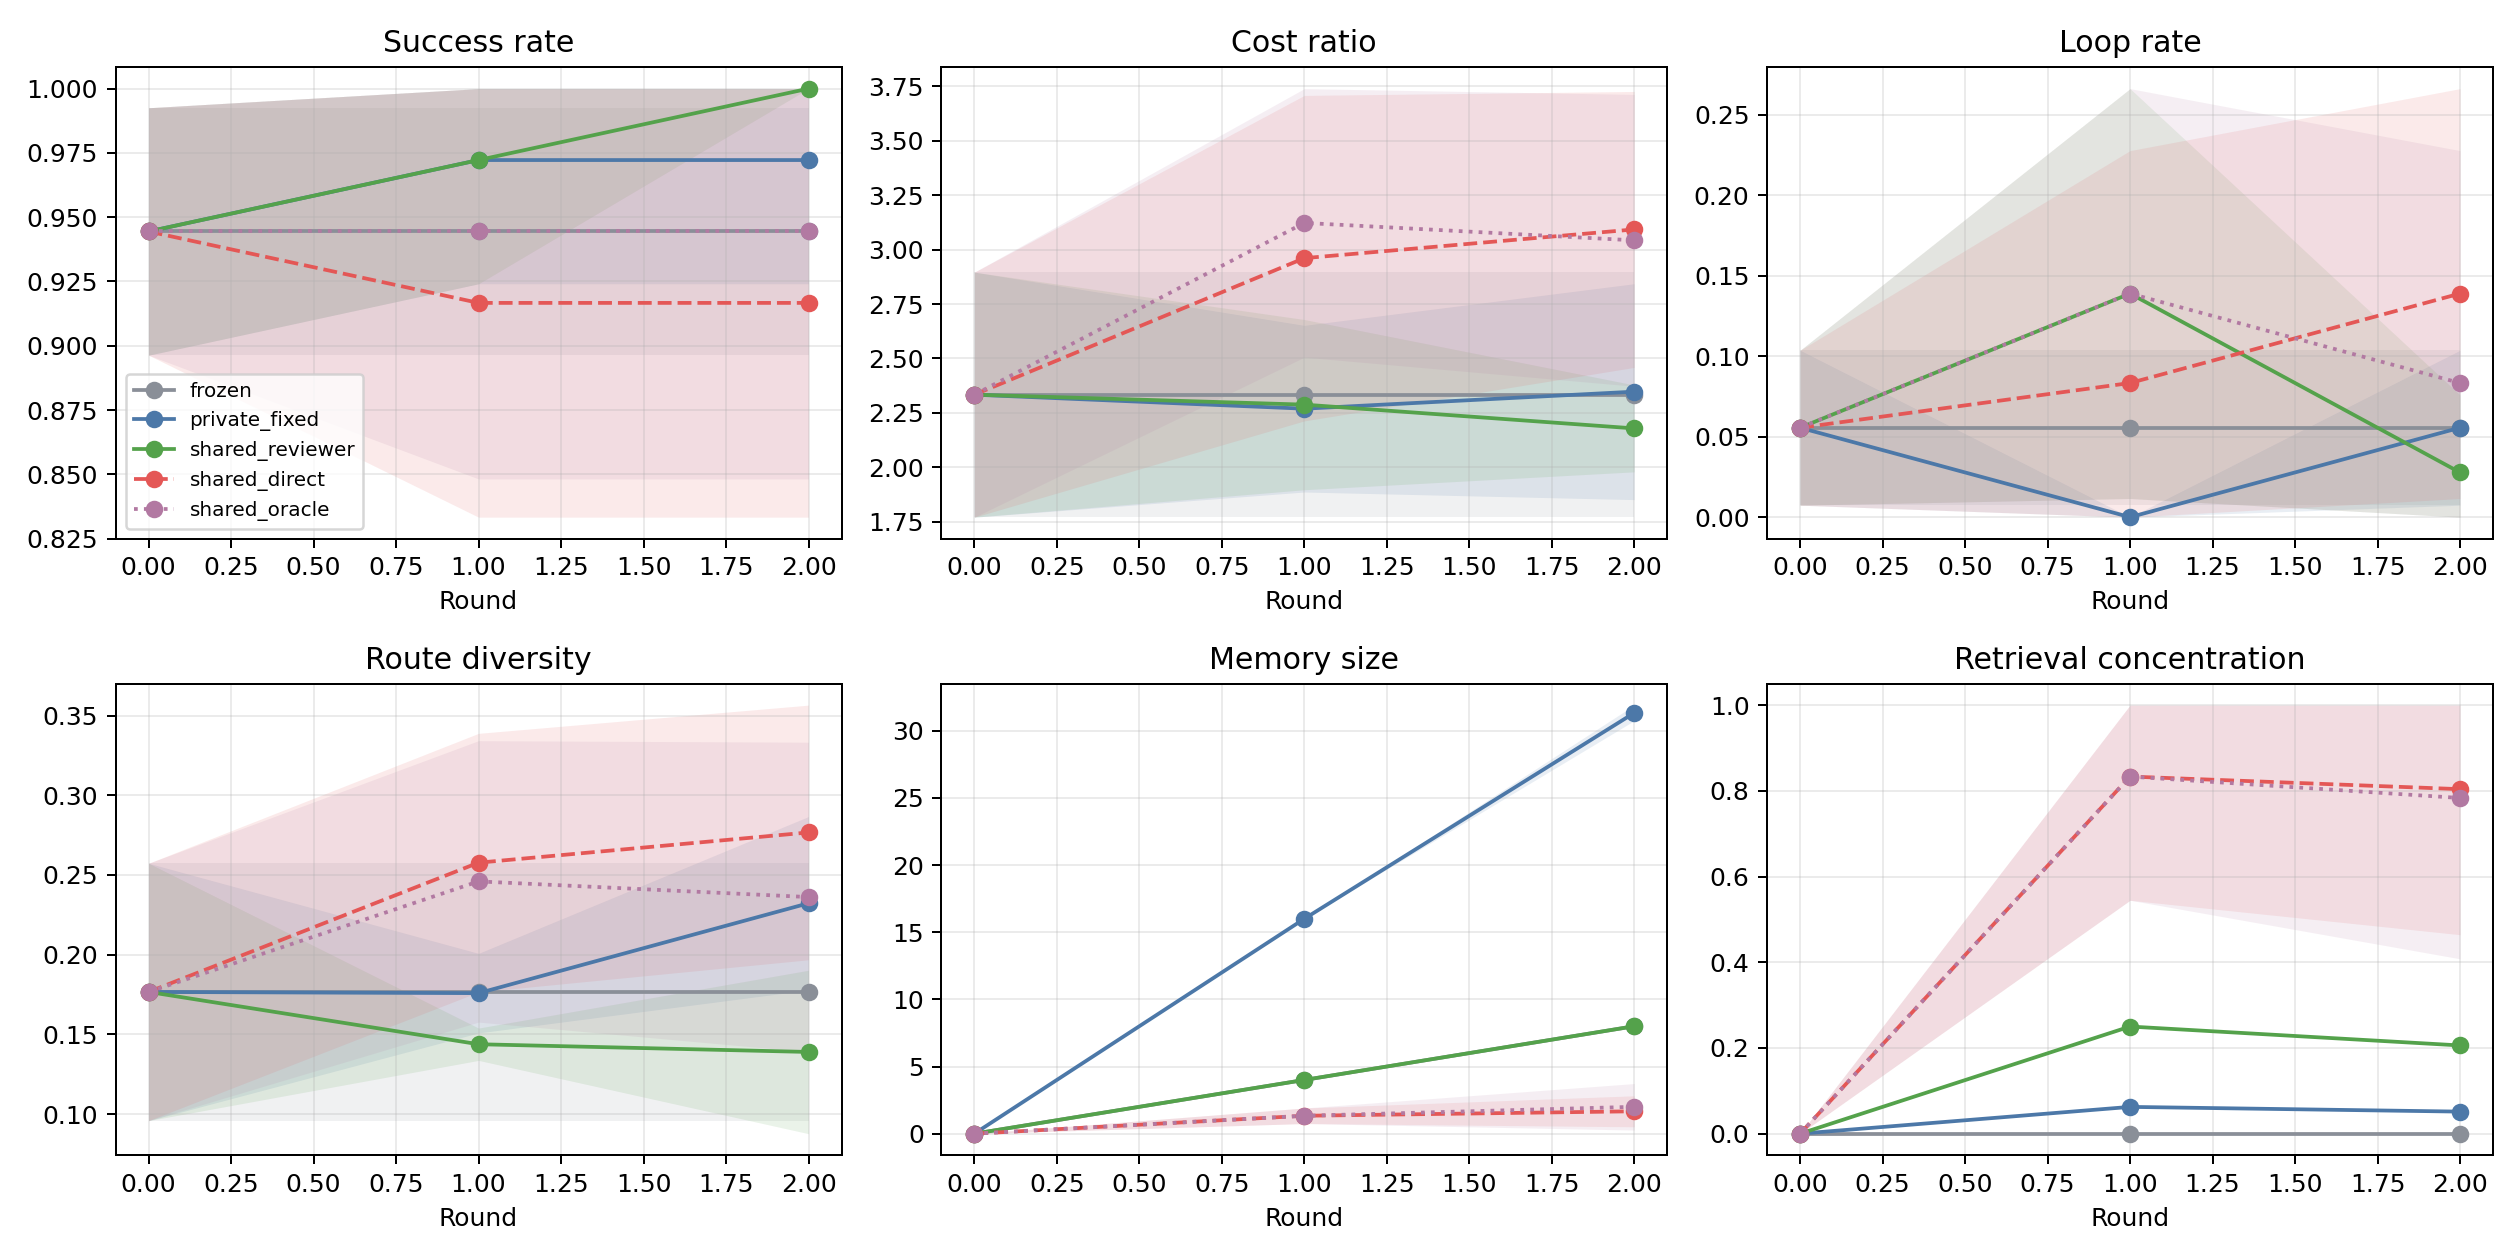
\includegraphics[width=\linewidth]{full_matrix_curves.png}
\caption{Full $T=3$ matrix. Shared reviewer improves short-horizon performance but compresses route diversity; direct/oracle memories produce higher cost and higher retrieval concentration.}
\label{fig:full-matrix}
\end{figure}

\section{Mechanism: Retrieval Concentration and Provenance}

The mechanism analysis supports the view that degradation is tied to concentrated reuse rather than merely to the existence of memory. Across active-memory rounds, retrieval concentration correlates positively with cost ratio ($r=0.663$) and stagnation rate ($r=0.646$), with a weaker but positive relation to loop rate ($r=0.349$). This suggests that the system becomes brittle when many agents repeatedly retrieve the same small set of memories.

\begin{figure}[h]
\centering
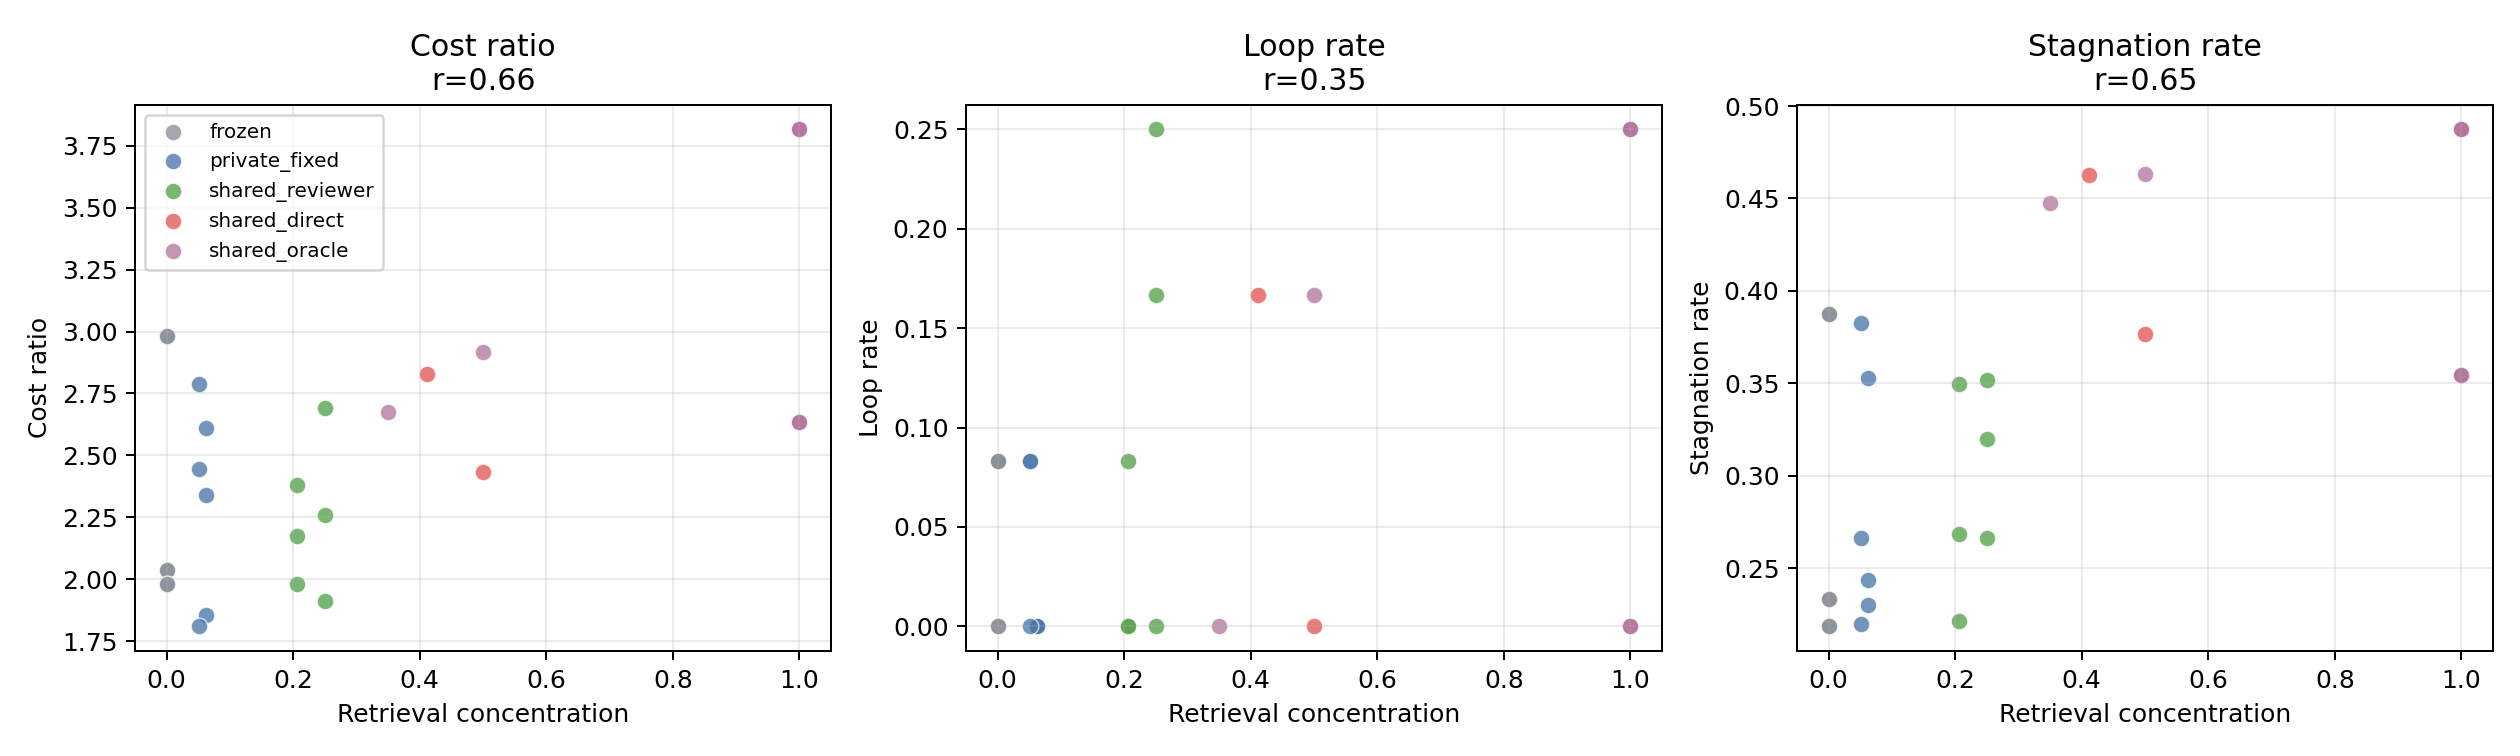
\includegraphics[width=\linewidth]{mechanism_scatter.png}
\caption{Retrieval concentration is positively associated with cost and stagnation in the current pilot. Each point is a condition/seed/round after memory becomes active.}
\label{fig:mechanism-scatter}
\end{figure}

Memory provenance further clarifies the failure mode. The most-retrieved shared direct and oracle memories are not false statements. For example, the top memory says to prefer actions that reduce distance while avoiding revisits and to submit once the goal is reached. Nevertheless, this memory can be sourced from successful but inefficient trajectories with source cost above 5, and some high-retrieval memories originate from failed or highly stagnant episodes. Thus, semantically correct text can still encode poor strategic provenance.

\begin{figure}[h]
\centering
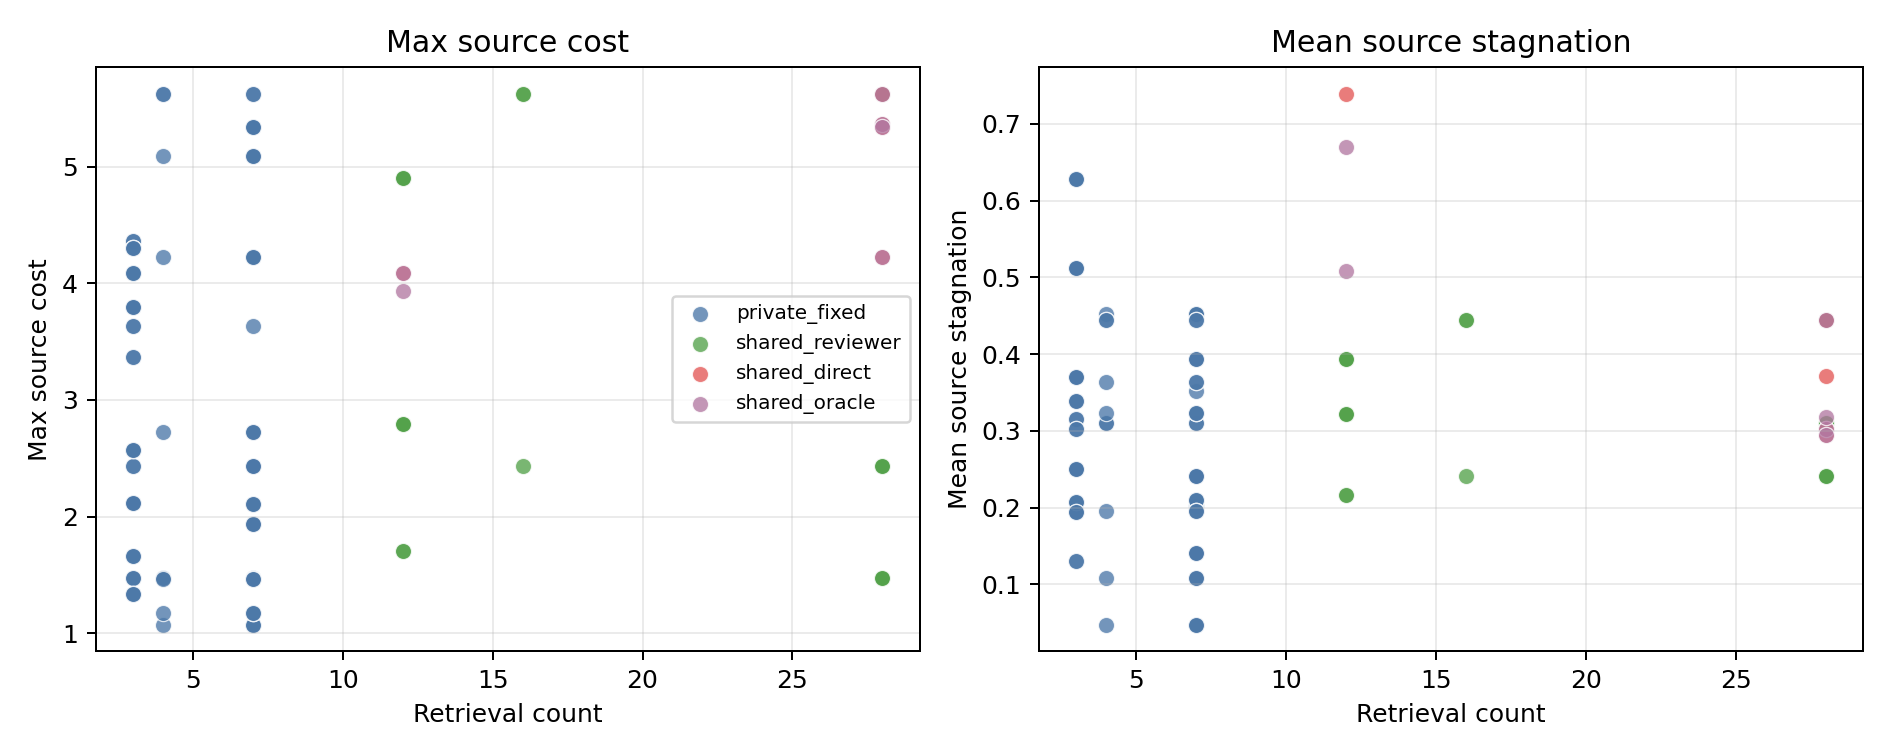
\includegraphics[width=0.86\linewidth]{provenance_scatter.png}
\caption{High-retrieval memories can have poor provenance. Direct/oracle memories are retrieved many times even when their source trajectories have high cost or high stagnation.}
\label{fig:provenance}
\end{figure}

\section{Longer Feedback Horizon: T=5 Targeted Stress}

The $T=5$ targeted stress test extends the feedback horizon for three conditions: frozen, shared reviewer, and shared direct. The frozen control remains unchanged across rounds. Shared reviewer initially improves performance at $t=1$ and $t=2$, but then degrades at $t=3$ and $t=4$: cost rises from 2.381 to 3.239 and loop rate rises to 0.167. Shared direct shows the clearest collapse: by $t=4$, success drops to 0.500, cost rises to 4.135, and loop rate reaches 0.917.

\begin{table}[h]
\centering
\caption{Final round of the $T=5$ targeted stress test for seed 0.}
\label{tab:t5}
\begin{tabular}{lrrrrrr}
\toprule
Condition & Success & Cost & Loop & Diversity & Memory & Retrieval conc. \\
\midrule
Frozen          & 0.917 & 2.982 & 0.083 & 0.264 & 15.0 & 0.000 \\
Shared reviewer & 0.917 & 3.239 & 0.167 & 0.257 & 15.0 & 0.183 \\
Shared direct   & 0.500 & 4.135 & 0.917 & 0.271 & 3.0  & 0.714 \\
\bottomrule
\end{tabular}
\end{table}

\begin{figure}[h]
\centering
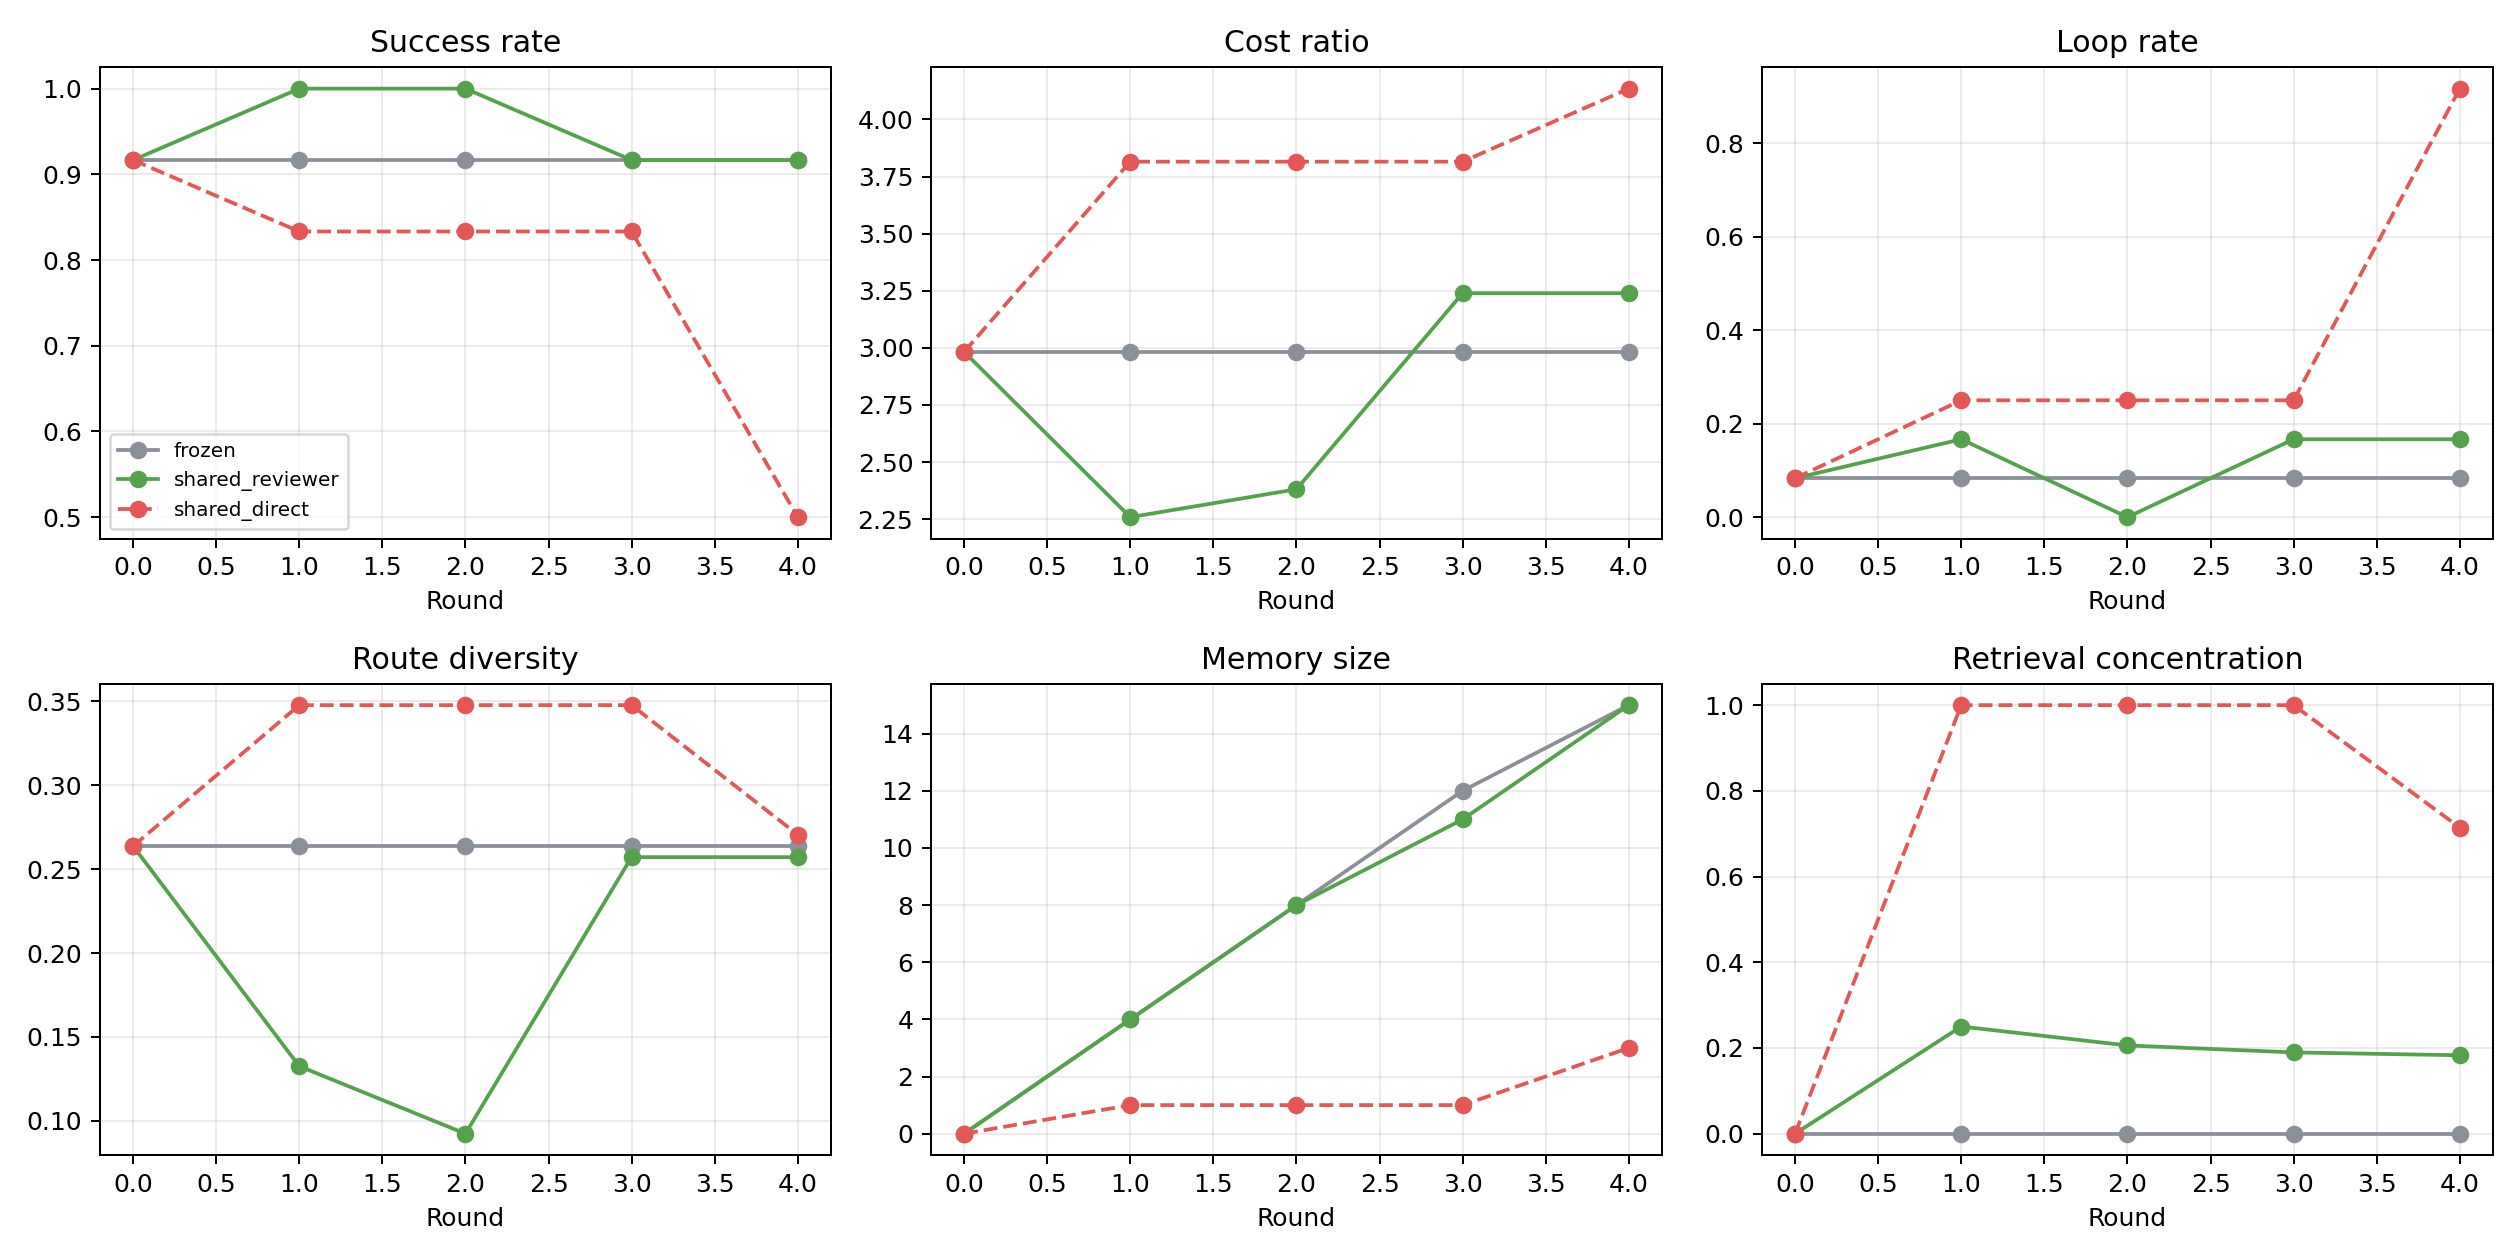
\includegraphics[width=\linewidth]{targeted_t5_curves.png}
\caption{The $T=5$ stress test exposes longer-horizon strategy degradation. Shared direct transitions from inefficient reuse to loop-heavy collapse; shared reviewer also loses its early advantage after additional experience iterations.}
\label{fig:t5-curves}
\end{figure}

\section{Case Study: No-Error Ant-Mill-Like Loop}

Figure~\ref{fig:t5-case} shows a representative $T=5$ case on the same heldout maze, round 4, agent 2. The shortest path length is 30. Frozen succeeds in 67 steps without a loop. Shared reviewer succeeds in 79 steps. Shared direct also eventually succeeds, but takes 148 steps, has cost ratio 4.93, revisit maximum 34, stagnation rate 0.736, and is flagged as looped. This is the desired ``no-error'' failure mode: the agent does not pass through walls and does not submit a wrong answer; instead, locally plausible strategy reuse yields excessive legal motion and repeated-state behavior.

\begin{figure}[h]
\centering
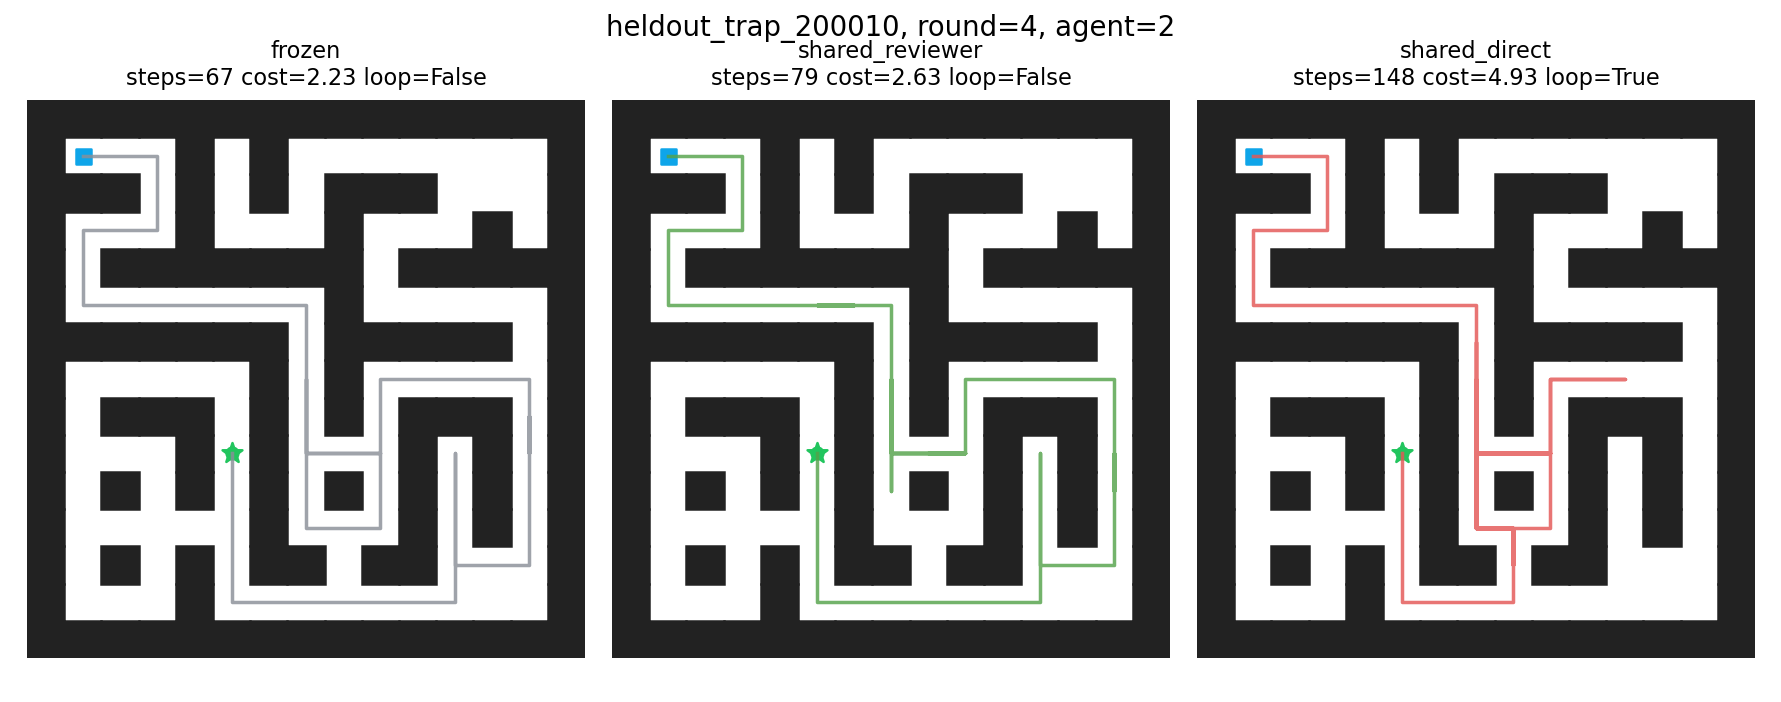
\includegraphics[width=\linewidth]{targeted_t5_case.png}
\caption{A $T=5$ mechanism case. Shared direct completes the maze but exhibits ant-mill-like legal looping: 148 steps for a 30-step shortest path, revisit maximum 34, and loop flag true.}
\label{fig:t5-case}
\end{figure}

\section{Interpretation}

These results suggest four preliminary findings. First, shared experience is not inherently harmful: reviewer-written shared memory can improve short-horizon performance. Second, direct or oracle-style shared memories can degrade efficiency despite being correct at the textual level. Third, retrieval concentration is a useful mechanism variable: high concentration predicts higher cost and stagnation. Fourth, longer feedback horizons reveal degradation that short runs can hide. This supports the ant-mill analogy: agents do not need to learn false facts to enter a global failure mode; locally valid traces can become collectively harmful when over-amplified through shared memory.

\section{Limitations and Next Steps}

This is a pilot rather than a final benchmark result. The $T=3$ matrix uses three seeds and small heldout sets; the $T=5$ stress test currently uses one seed. The next step is to repeat the $T=5$ targeted stress over additional seeds and then bridge the mechanism to a tool-use or web-task environment where shortest paths are unavailable but cost, repeated state/action, tool calls, tokens, and time-to-success can play analogous roles. We should also test mitigation mechanisms such as provenance-aware retrieval, memory diversity regularization, and reviewer prompts that explicitly penalize high-cost source trajectories.

\end{document}
